\documentclass[10pt,a4paper,landscape]{article}
\usepackage{multicol}
\usepackage{calc}
\usepackage{ifthen}
\usepackage[landscape]{geometry}
\usepackage{amsmath,amsthm,amsfonts,amssymb,mathtools}
\usepackage{color,graphicx}
\usepackage{hyperref}
\usepackage{listings}
\usepackage{underscore}
\usepackage{todonotes}
\usepackage{algpseudocode}
\usepackage{algorithm}

% Cheatsheet style
% Cheatsheet style

% This sets page margins to .5 inch if using letter paper, and to 1cm
% if using A4 paper. (This probably isn't strictly necessary.)
% If using another size paper, use default 1cm margins.
\ifthenelse{\lengthtest{\paperwidth = 11in}}
  % Then
  { \geometry{top=.5in,left=.5in,right=.5in,bottom=.5in} }
  % Else
  { \ifthenelse{\lengthtest{\paperwidth = 297mm}}
    {\geometry{top=1cm,left=1cm,right=1cm,bottom=1cm} }
    {\geometry{top=1cm,left=1cm,right=1cm,bottom=1cm} }
  }

% Turn off header and footer
\pagestyle{empty}

% Redefine section commands to use less space
\makeatletter
\renewcommand{\section}{\@startsection{section}{1}{0mm}%
                                {-1ex plus -.5ex minus -.2ex}%
                                {0.5ex plus .2ex}%x
                                {\color{darkred}\normalfont\large\bfseries}}
\renewcommand{\subsection}{\@startsection{subsection}{2}{0mm}%
                                {-1explus -.5ex minus -.2ex}%
                                {0.5ex plus .2ex}%
                                {\color{darkdarkred}\normalfont\normalsize\bfseries}}
\renewcommand{\subsubsection}{\@startsection{subsubsection}{3}{0mm}%
                                {-1ex plus -.5ex minus -.2ex}%
                                {1ex plus .2ex}%
                                {\normalfont\small\bfseries}}
\makeatother

% Define BibTeX command
\def\BibTeX{{\rm B\kern-.05em{\sc i\kern-.025em b}\kern-.08em
    T\kern-.1667em\lower.7ex\hbox{E}\kern-.125emX}}

% Don't print section numbers
\setcounter{secnumdepth}{0}

\setlength{\parindent}{0pt}
\setlength{\parskip}{0pt plus 0.5ex}

% Setting colors
\definecolor{lightgray}{rgb}{0.7,0.7,0.7}
\definecolor{lightergray}{rgb}{0.9,0.9,0.9}
\definecolor{darkblue}{rgb}{0.4,0.4,1}
\definecolor{darkred}{rgb}{0.9,0.2,0.2}
\definecolor{darkdarkred}{rgb}{0.6,0.0,0.0}
\definecolor{lightred}{rgb}{1,0.6,0.6}
\definecolor{lightgreen}{rgb}{0.6,1,0.6}
\definecolor{lightblue}{rgb}{0.6,0.8,1}
\definecolor{darkgreen}{rgb}{0.4,1,0.4}

% Set code listing style
\lstset {
    backgroundcolor=\color{lightgray},
    basicstyle=\ttfamily\scriptsize,
    breaklines=true,
}

\lstdefinestyle{bb}{
    backgroundcolor=\color{lightergray},
    frame=L,
    xleftmargin=\parindent,
}

% Remove `itemize` indentation
\usepackage{enumitem}
\setlist[itemize]{leftmargin=*}

% Set hyperlink style
\hypersetup{hidelinks}

% Enable figures
\newenvironment{colfig}
  {\par\medskip\noindent\minipage{\linewidth}}
  {\endminipage\par\medskip}

% Enable arg min/max math operators
\DeclareMathOperator*{\argmin}{arg\,min}
\DeclareMathOperator*{\argmax}{arg\,max}


% Shorthands
\renewcommand{\bf}[1]{\ensuremath{\mathbf{#1}}}
\newcommand{\E}{\mathrm{E}}
\newcommand{\Var}{\mathrm{Var}}
\newcommand{\Cov}{\mathrm{Cov}}
\newcommand{\balpha}{\boldsymbol\alpha}
\newcommand{\bbeta}{\boldsymbol\beta}
\newcommand{\bdelta}{\boldsymbol\delta}
\newcommand{\btheta}{\boldsymbol\theta}
\newcommand{\bPhi}{\boldsymbol\Phi}
\newcommand{\code}{\mathcal{C}}
\newcommand{\alphabet}{\mathcal{U}}

\pdfinfo{
  /Title (Machine Learning Cheat Sheet)
  /Creator (TeX)
  /Producer (pdfTeX 1.40.0)
  /Author (Dennis Meier)
  /Subject (Machine Learning cheatsheet)
  /Keywords (machinelearning, ml, bayes, regression, classification)
}

% -----------------------------------------------------------------------

\begin{document}
\title{Information Theory Cheat Sheet}

\raggedright
\footnotesize
\sffamily
\begin{multicols*}{4}

% multicol parameters
% These lengths are set only within the two main columns
%\setlength{\columnseprule}{0.25pt}
\setlength{\premulticols}{1pt}
\setlength{\postmulticols}{1pt}
\setlength{\multicolsep}{1pt}
\setlength{\columnsep}{2pt}

\begin{center}
\Large{\underline{Information Theory Cheat Sheet}}
\end{center}

% ----------


\section{Entropy and co.}
\begin{colfig}
\centering
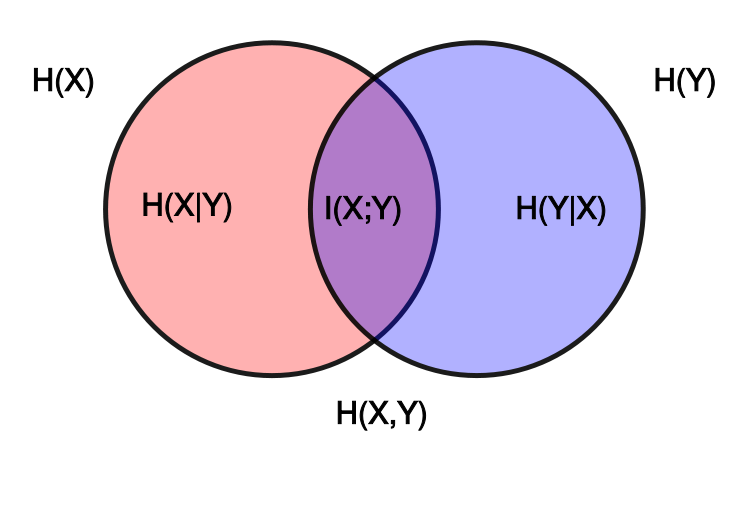
\includegraphics[width=\linewidth]{entropy-quantities-venn-diagram.png}
\end{colfig}

\subsection{Entropy}

$H(U) = \sum_u - P(u) \log_2(P(u)) = E[- \ln(P(U))]$

\subsubsection{Properties:}
\begin{itemize}
	\item $H(U) \leq \log | \alphabet |$ with equality if all elements in $\alphabet$ are equally probable.
	\item $H(U) \geq 0$ always.
	\item $H(U) \geq H(f(U))$
\end{itemize}

\subsection{Joint Entropy}
$H(X,Y) = H(X) + H(Y | X) = H(Y) + H(X | Y)$

\subsubsection{Properties:}
\begin{itemize}
	\item Joint increases entropy: $H(X, Y) \geq H(X)$ with equality iff $X$ and $Y$ are independent.
	\item $H(X,Y) \leq H(X) + H(Y)$
	\item Chain rule: $H(X, Y) = H(X) + H(Y | X)$
	\item General chain rule: $H(X_1, X_2, ..., X_n) = \sum_{i=1}^n H(X_i | X_1, ..., X_{i-1})$
\end{itemize}


\subsection{Conditional Entropy}

$H(U | V = v) = \sum_u - P(u | v) \log P(u | v)$

$H(U | V) = \sum_v P(v) H(U | V = v)$


\subsubsection{Properties:}
\begin{itemize}
	\item Conditioning reduces entropy: $H(U | V) \leq H(U)$
	\item $H(U | V) \leq H(U | f(V))$ since $U, V, f(V)$ form a markov chain.
	\item Chain rule: $H( U | V) = H(U,V) - H(V)$
	\item If $X_i$ is a stationary stochastic process: $H(X_n | X^{n-1}) \leq H(X_i | X^{i-1})$ with $i \in 1, ..., n$
\end{itemize}

\subsubsection{Fano's Inequality}
Suppose $U,V$ are random variables with the same alphabet. Let $p=Pr(U \neq V)$. Then $ H(U|V) \leq h_2(p) + p\log (|\mathcal{U}|-1)$ where $h_2(p) = p\log \frac{1}{p} + (1-p)\log\frac{1}{1-p}$

\subsection{Mutual Information}
\begin{align*}
I(U; V) &= H(U) + H(V) - H(U,V)\\
		&= H(U) - H(U | V)\\
		&= H(V) - H(V | U)\\
		&= H(U,V) - H(U | V) - H (V | U)
\end{align*}

\subsubsection{Properties:}
\begin{itemize}
	\item Nonnegative: $I(U;V) \geq 0$ with equality if $U, V$ ar independent.
	\item Chain rule: $I(X; Y, Z) = I(X;Z) + I(X; Y | Z)$
	\item General chain rule for mutual Information: $I(X_1, ..., X_n; Y) = \sum_{i=1}^n I(X_i; Y | X_1, ..., X_{i-1})$
	\item Data processing inequality: $I(X,Y) \geq I(X, Z)$ if X, Y, Z form a markov-chain.
	\item Symmetric: $I(X;Y) = I(Y;X)$.
\end{itemize}

\subsection{Conditional Mutual Information}
\begin{align*}
I(X;Y|Z) 	&= I(X;Y,Z) - I(X;Z)\\
			&= H(X,Z) + H(Y,Z) - H(X,Y,Z) - H(Z)\\
			&= H(X|Z) - H(X|Y,Z)\\
			&= \sum_z p(z) I(X;Y|Z=z)
\end{align*}
\subsection{Cross-Entropy}
$$ D(p || q) = \sum_x p(x) \log \frac{p(x)}{q(x)}$$

\section{Entropy Rate \& Typical Sets}
Entropy rate of a stochastic Process $\{X_i\}$ is

$$H(X_i) = \lim_{n \rightarrow \infty} \frac{1}{n} H(X_1, X_2, ..., X_n)$$

If a process is stationary, then the entropy rate exists and is equal to:

$$H(X_n | X_{n-1}, X_{n-2}, ..., X_1)$$

\subsection{Asymptotic Equpartition Property}
Information Theory's analog to the law of large numbers: If $X_1, X_2, ...$ are i.i.d. $\sim p(x)$, then
$$ - \frac{1}{n} \log p(X_1, X_2, ..., X_n) \rightarrow H(X) \text{ in probability}$$

Or alternatively,

$$ p(X_1, X_2, ..., X_n) \rightarrow 2^{-n H}$$

\subsection{Typcial Set}
The typical set $T_\epsilon$ is the set of sequences $(x_1, x_2, ..., x_n) \in \alphabet^n$ with empirical entropies $\epsilon$-close to the true entropy of $X$:

\begin{align*}
	&p(x_1, x_2, ..., x_n) = 2^{-n(H(X) \pm \epsilon)}\\
	\Leftrightarrow & - \frac{1}{n} \log p(x^n) = H(X) \pm \epsilon\\
	\Leftrightarrow &\left | - \frac{1}{n} \log p(x^n) - H(X) \right | < \epsilon
\end{align*}

\subsubsection{Properties of the typical set:}
\begin{itemize}
	\item Has probability nearly 1: $P(T_\epsilon) > 1 - \epsilon$
	\item All elements in $T_\epsilon$ are nearly equiprobable (with probability as given above)
	\item The number of elements in $T_\epsilon$ is nearly $2^{nH}$
\end{itemize}

\section{Coding schemes}
\subsection{Tunstall Coding}

\begin{algorithmic}[1]
\State {$D$ := tree of $|\mathcal{U}|$ leaves, one for each letter in $\mathcal{U}$.}
\While{$|D| < C$}
	\State {Convert most probable leaf to $|\mathcal{U}|$ sub-leaves.}
\EndWhile
\end{algorithmic}

\subsection{Huffman Coding}

\begin{algorithmic}[1]
\State {Leaf node for each symbol in $\mathcal{U}$, add it to the priority queue.}
\While {there is more than one node in the queue}:
	\State {Remove the two nodes of highest priority (lowest probability) from the queue}
	\State {Create a new internal node with these two nodes as children and with probability equal to the sum of the two nodes' probabilities.}
	\State {Add the new node to the queue.}
\EndWhile
\State {The remaining node is the root node and the tree is complete.}
\end{algorithmic}

\subsection{Lempel-Ziv coding}
\begin{algorithmic}[1]
	\State {Set $\mathcal D = \alphabet$}
	\Loop
		\State Associate to each $w \in \mathcal D$ a $\lceil \log | \mathcal D | \rceil$-bit binary representation, based on dictionary order.
		\State Parse the next work $w$ from the source sequence using $\mathcal D$
		\State Set $\mathcal D \gets \mathcal D \setminus \{w\} \cup \{ w u: u \in \alphabet \}$
	\EndLoop
\end{algorithmic}

\subsection{Hamming Code}
\todo{Fill and maybe move to linear codes}

\section{Source Coding}
A source code $\code$ for a random variable $X$ is a mapping from the range of X to $D^*$, the set of finite-length strings of symbols from a D-ary alphabet.

Expected length of a source code C(x) for a random variable X with probability mass function p(x) is given by:
$$L(C) = \sum_{x \in \alphabet} p(x) l(x) \geq H(X)$$
with equality only if $D^{-l_i} = p_i$.

Expected codeword length: $E[len(\code(U))] < H(U) + 1$

Prefix-free codes can always be represented as leaves of a full tree.

\begin{colfig}
	\centering
	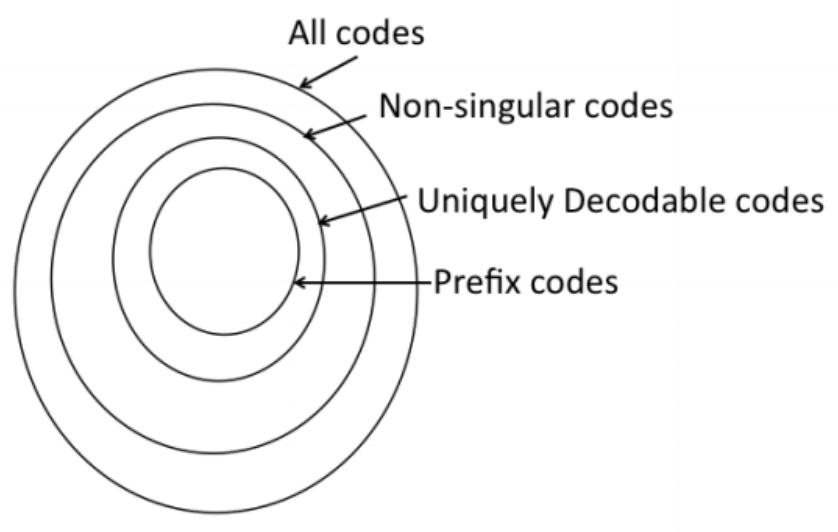
\includegraphics[width=\linewidth]{code-classes.png}
\end{colfig}

\subsection{Kraft's inequality}
$$\sum_{u \in \alphabet} 2^{-len(\code(u))} \leq 1$$

$\code$ prefix free $\implies$ Kraft

$\code$ uniquely decodable $\implies$ Kraft

$l(u)$ fullfills Kraft $\implies$ $\exists \ \code$, prefix free with $len(\code(u)) = l(u)$

\subsection{Finite state machine}
A set of states $S$, a starting state, some state transfer function $g: S \times \alphabet \rightarrow S$ and some output function $f: S \times \alphabet \rightarrow \{0,1\}^*$

Letigimate FSM needs to be information lossless, i.e. $\forall s \in S$ $\forall u_1, ..., u_m \neq v_1, ..., v_m: g(s, \vec u) = g(s, \vec v) \implies f(s, \vec u) \neq f(s, \vec v)$

For a $L$-state finite state machine the compressibility is $\rho_M \geq 1/L$

A lempel-ziv procedure does at least as well as the best finite state machine there exists for a given sequence: $\rho_{LZ}(\vec x) \leq \rho_{FSM}(\vec x)$.

\section{Channel Coding}
\subsection{Discrete Memoryless Channels}
memoryless: $P(y|x, x_1^{i-1}, y_1^{i-1}) = p(y|x)$

without feedback if $P(x_i|x_1^{i-1},y_1^{i-1}) = P(x_i|x_1^{i-1})$

memoryless without feedback: $$P(y_1^n | x_1^n) = \prod_{i=1}^n p(y_i|x_i)$$
$$I(X_1^n;Y_1^n) \leq \sum_{i=1}^n I(X_i;Y_i) \leq nC$$

\subsection{Channel Capacity}
Information channel capacity of a discrete memoryless channel:
$$C = \max_{p(x)} I(X; Y)$$

Feedback does not increase the capacity for a discrete memoryless channel. Tinkering with the channel by using functions on it does not increase the capacity, either. However, channels with memory can have higher capacity than without memory.

\subsubsection{Properties}
\begin{enumerate}
	\item Positive: $C \geq 0$ since $I(X; Y) \geq 0$
	\item $C \leq \log | \mathcal{X} |$ since $C = \max I(X; Y) \leq \max H(X) =  \log | \mathcal{X} |$ and similar for Y.
\end{enumerate}

The capacity subject to a cost constraint $\beta$ and a cost function $b(x)$ changes the definition to $C = \max_{p(x): E[b(X)] < \beta} I(X; Y)$

\subsection{Transmission}
\begin{colfig}
	\centering
	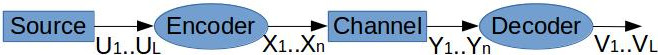
\includegraphics[width=\linewidth]{comm-setup.png}
\end{colfig}

Source produces a letter each $\tau_S$ sec and channel accepts input symbols every $\tau_C$ sec: $\tau_S L = \tau_C n$

Suppose $U_1U_2..$ is a stationary source with Entropy Rate $\mathcal{H}$, and we have the setup above, then $\frac{1}{L} H(U_1..U_L|V_1..V_L) \geq \mathcal{H} - \frac{n}{L}C = \tau_S\left(\frac{\mathcal{H}}{\tau_S}-\frac{C}{\tau_C}\right)$

No matter how encoder and decoder are designed:
$$ h_2(\bar{P_e}) + \bar{P_e}\log(|\mathcal{U}|-1) \geq \tau_S \left(\frac{\mathcal{H}}{\tau_S}-\frac{C}{\tau_C}\right)$$ with $\bar{P_e} = \frac{1}{L} \sum_{i=1}^L P(U_i \neq V_i)$

Bad news: if $\frac{\mathcal{H}}{\tau_S} > \frac{C}{\tau_C}$ then $\bar{P_e}$ not arbitrary small

Good news: if $\frac{\mathcal{H}}{\tau_S} < \frac{C}{\tau_C}$ can achieve $\bar{P_e} \rightarrow 0$

\subsection{Channel Coding Theorem}
$M$ is the number of different messages we can send over the channel.
$R = \frac{\log M}{n}$ is the rate of the channel code, i.e. how many message bits are encoded per channel bit sent.

For a discrete memoryless channel, all rates below capacity $C$ are achievable. Specifically, for every rate $R < C$ there exists a sequence of $(2^{nR}, n)$ codes with maximum probability of error $\rightarrow 0$.

Conversely, any sequence of $(2^{nR}, n)$ codes with a maximum error probability going to zero must have $R \leq C$.

\subsection{Source-channel theorem}
A stochastic process with entropy rate H cannot be sent reliably over a discrete memoryless channel if $H > C$. Conversely, if the process satisfies the asymptotic equipartition property (APP), the source can be transmitted reliably if H < C.

\section{Example Channels}
\subsection{Binary Symmetric channel}
$C = 1 - H(p)$ because:
\begin{align}
	I(X; Y) &= H(Y) - H(Y | X)\\
			&= H(Y) - \sum p(x) H(Y| X = x)\\
			&= H(Y) - \sum p(x) H(p)\\
			&= H(Y) - H(p)\\
			&\leq 1 - H(p).
\end{align}
\begin{colfig}
	\centering
	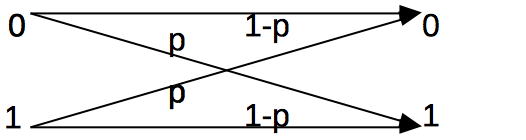
\includegraphics[width=0.6\linewidth]{binary-symmetric-channel.png}
\end{colfig}

\subsection{Binary erasure channel}
$C = 1 - \alpha$

\subsection{Arbitrary symmetric channel}
A channel is said to be \emph{weakly symmetric} if every row of the transition matrix $p(\cdot | x)$ is a permutation of every other row and all the column sums $\sum_x (y|x)$ are equal. For weakly symmetric channels:
$C = \log | \mathcal{Y} | - H(\text{row of transition matrix})$
and this is achieved by a uniform distribution on the input alphabet.

\section{Differential Entropy}
$$h(X) = -\int_\mathbb{X} f(x)\log f(x)\,dx$$

\subsection{Examples}
\begin{itemize}
	\item For the uniform distribution $\mathcal{U}[0, a]$:
	$h(X) = - \int_0^a \frac{1}{a} \log \frac{1}{a} dx = \log a$
	\item For the normal:
	$h(X) = \frac{1}{2} \log 2 \pi e \sigma$
\end{itemize}


\subsection{Properties:}
\begin{itemize}
	\item General chain rule: $h(X_1, \ldots, X_n) = \sum_{i=1}^{n} h(X_i|X_1, \ldots, X_{i-1}) \leq \sum h(X_i)$
	\item Translation-Invariant: $h(X + c) = h(X)$
	\item Scalable: $h(aX) = h(X) + log|a|$
	\item Conditioning reduces Entropy: $h(X|Y) \leq h(X)$ with equality iff $X$ and $Y$ are independent.
	\item Can be negative, unlike discrete entropy.
	\item Entropy of X (on $\mathbb{R}$ with zero mean and variance $\sigma^2$) is upper bounded by: $h(X) \leq \frac{1}{2} \log ( 2\pi e \sigma^2)$, with equality if $X$ is a Gaussian.
	\item Entropy of X (on $[0, \infty]$ with mean $\lambda$) is upper bounded by $h(X) \leq \ln(\lambda) + 1$ with equality if X is exponentially distributed $p(X) = \frac{1}{\lambda} e^{-x/\lambda}$
	\item Entropy of X (on $[0, a]$) is bounded by $h(X) \leq \log a$, with equality if $X$ is Uniform.
\end{itemize}





\section{Utilities}
$\log(x) \leq 1 + x$

$\lceil x \rceil < 1 + a$

$E[Z] = \sum_{n=0}^{\infty} Pr[Z > n]$

Jensen's inequality for convex functions $f$: $ E[f(X)] \geq f(E[X])$

$a^b = 2^{ b \log a}$

Law of large numbers: $\lim_{n \rightarrow \infty} \frac{1}{n} \sum_{i=1}^n X_i = E[X]$

If a $K$-ary tree has $\alpha$ intermediate nodes, the tree has $1+(K-1)\alpha$ leaves.


$\max(f(t) + g(t)) \leq \max(f(t)) + \max(g(t))$


$h_2 \left(\frac{1}{L}\sum_{i=1}^L p_i \right) \geq \frac{1}{L} \sum_{i=1}^L h_2(p_i)$

Normal distribution: $f(x \; | \; \mu, \sigma) = \frac{1}{\sigma\sqrt{2\pi} } \; e^{ -\frac{(x-\mu)^2}{2\sigma^2} }$

\subsection{Convexity}

$f$ is convex if: $f((1-t)x+ t y)\leq (1-t) f(x)+ t f(y)$

Let $\{f_i\}$ be a set of convex functions and $c_i \geq 0 \ \forall i$:
Then $\sum_{i=1}^n c_i f_i(x_i)$ is convex.

$f(x) = \sup_{i \in I} f_i(x)$ is convex.

$g(x) = h \circ f$ is convex if $f(x)$ is bounded and convex and $h(x)$ is increasing and convex.
\end{multicols*}
\end{document}
